%%
%%
%% This file should be edited by user
%%

\chapter{tinyos} \label{chapter:tinyos}

\section{What is tinyOS}

tinyOS is a free and open operating system for hardware motes, which is written in nesC. Development started as a collaboration of Berkeley University with Intel Research and Crossbow Technology, a california based company.

A hardware mote is a microcontroller based node in a wireless sensor network, capable of reading sensory information, processing and exchanging of this data with other nodes. Communication typically goes on over wireless networks.

One of tinyOS's most important features is that tinyOS applications are built out of components, which are connected or wired to each other by interfaces. 

\section{History}

Developement of tinyOS started in 1999 at Berkeley university. The first supported platform was a mote 
called 'WeC', as shown in figure~\ref{fig:WeC}. For communication, this platform is equipped wit an radio device and SPI and UART - interfaces. As cpu an Atmel AVR AT90LS8535 microprocessor, clocked with 4MHz, is used. A major advantage of this mote is that it can be programmed over the wireless interface.
\begin{figure}[h]
 \centerline{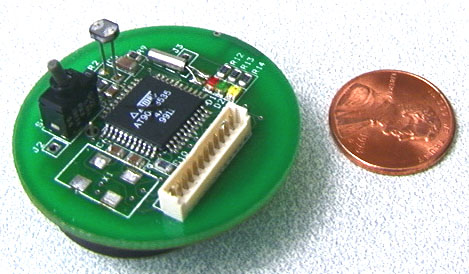
\includegraphics[width=.5\columnwidth]{pics/WeC.png}}
  \caption{WeC Mote}
  \label{fig:WeC}
\end{figure}

In the next years, the 'rene' and 'mica' platforms are developed. In the year 2002, work on the nesC programming language began. Until that, tinyOS consisted of a mixture of C files and Perl scripts. In the same year, tinsOS 1.0, the first tinyOS implemented in nesC, is released. 

Improvement of tinyOS 1.x went on until february 2006, when tinyOS 2.0 beta1 was released. Version 2.1 was finished in april 2007. Among numerous bugfixes, a cc2420 wireless radio stack implementation was added in this release. tinyOS 2.02 was released some months later, which included an cc2420 stack reimplementation and bugfixes.
After that, in august 2008, support for the 'iris' and 'shimmer' platforms was added by distribution of version 2.1. Clearly, bugfixes were included in this release too.

At the time of this writing, the latest tinyOS version is 2.1.1, which was released in April 2010. Most important add-ons are support for the 'mulle', 'epic' and 'shimmer2' - platforms. 

\section{Supported Platforms}

With version 2.1.1, a range of hardware motes are supported out-of-the-box. A brief description of this platforms and its most important communication devices are given in the following list. Obviously, most of this platforms provide interfaces for UART, I2C, SPI or others peripherals, depending of the microcontroller and extension boards used, too. These features are not listed here.

\begin{itemize}
 \item btnode3: Atmega128L cpu and radio/bluetooth communication devices
 \item epic: MSP430 cpu and CC2420 radio chip
 \item eyesIFX: MSP430F149/F1611 and TDA5250 wireless transceiver
 \item intelmote2: PXA271 XScale cpu and CC2420 radio chip 
 \item mica: Atmega103 and TR1000 radio chip
 \item mica2: Atmeage128L and Chipcon 868/916 radio chip
 \item mica2dot: Atmega128 and cc1000 transceiver
 \item micaz: Atmega128 and cc2420 radio chip
 \item mulle: Renesas M16C and AT86RF230 transceiver
 \item sam3s\_ek: SAM3S4C chip and cc2520 transceiver
 \item sam3u\_ek: SAM3S4C chip and cc2420 transceiver
 \item shimmer / shimmer2 / shimmer2r : MSP430 cpu and CC2420 transceiver
 \item span: MSP430 cpu and CC2420 transceiver
 \item telosa / telosb: MSP430 cpu and CC2420 transceiver
 \item tinynode: MSP430 cpu and Semtech SX1211 transceiver
 \item ucmini: Atmega128RFA1 cpu(low power transceiver cpu integrated)
 \item z1: MSP430 cpu and CC2420 transceiver
\end{itemize}

\section{tinyOS hardware abstraction}

When looking at the supported hardware platforms, one can see that many platforms use the same cpu and/or communication hardware. To avoid rewriting of code, hardware abstraction is used.
By introducing hardware abstraction, it is easier to port applications from one platform to another, and application development itself gets easier too. On the other hand, abstraction means generalisation, which is problematic because hardware motes only have very limited resources and strict energy-efficiency requirements.
So, tinyOS uses a 3-level \textit{Hardware Abstraction Architecture} to provide a flexible and performant framework to build applications on, as shown in figure~\ref{fig:haa}.

\begin{figure}[h]
 \centerline{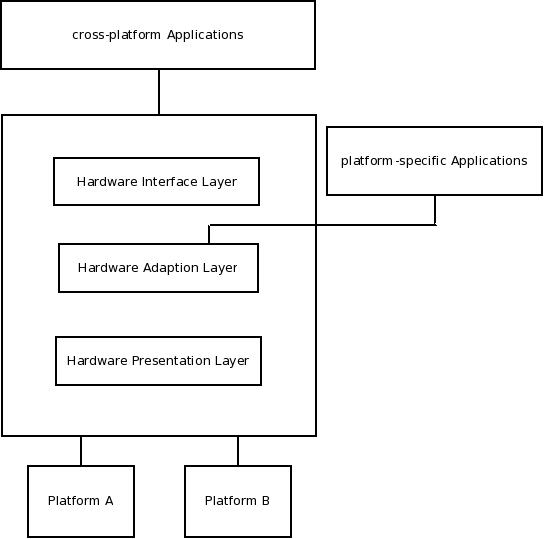
\includegraphics[width=.6\columnwidth]{pics/hardwareabstraction.png}}
  \caption{Hardware Abstraction Architecture}
  \label{fig:haa}
\end{figure}

In contrast to other embedded OS that use only 2 layer abstraction, the third tinyOS layer provides more flexibility. For maximum performance, a \textit{Platform-Specific-Application} can directly hook into the \textit{Hardware Adaption Layer}, circumventing the \textit{Hardware Interface Layer}.


\section{tinyOS internals}

\subsection{Basic - Scheduler}

By default, tinyOS 2.x uses a \textbf{non-preemptive FIFO} scheduler with a maximum of 255 parameterless tasks waiting for execution. A task can only be scheduled once at a time, if periodic execution is needed the task has to re-post itself just before finishing. The scheduler itself consists of an interminable for-loop, that pops ( = executes) one task after the other, in sequence as this tasks got pushed. If no tasks are waiting for execution, the scheduler enters a powersaveing-mode immediatly.

Because the scheduler of tinyOS is implemented as a component it is possible to replace this default FIFO-scheduler with a selfwritten one. See ~\cite{tep106:2003} for details how to implement a selfwritten scheduler.

\subsection{Microcontroller Power Management}

To reduce power consumption, a microcontroller should always run in the lowest power state possible. As mentioned above, tinyOS enters a low power mode if the task queue is empty. Normally, microcontrollers support a full range of low power modes, the ATmega128 - for example - supports up to 6 different power saving modes.
To decide what mode fits best, tinyOS uses the control- and statusregisters to find the proper lowpower-mode.

For example, on a ATmega128-based platform, the cpu-specific powersaving-mode \textit{IDLE} is to be choosen if one or more timer, SPI, UART or I2C are in use. If the ADC-submodule is working, another mode, \textit{ADC Noise Reduction}, is entered. If none of this modules are active, the cpu is set to \textit{POWER DOWN}, from which it only can resume by some external interrupts/resets or a SPI address match interrupt.


%%
%% = eof =====================================================================
%%
